\section{Protection Reverse Proxy}
\label{sec:proteciton-reverse-proxy}

Einen Web- oder Applikationsserver ``direkt'' im Internet zu platzieren ist mehr als unvorsichtig. Natürlich kann man den Server in einer DMZ hinter einer entsprechenden Firewall platzieren, was ihn auf dem Netzwerklayer vor Angriffen schützen kann. In Verbindung mit einem ``Protection Reverse Proxy'' kann der Server aber zusätzlich auch auf dem Applicationlayer geschützt werden.

\subsection*{Kontext}
Ein System, welches HTTP/HTTPS zur Kommunikation verwendet soll geschützt werden.

\subsection*{Problem}
Der Einsatz einer \nameref{sec:packet-filter-firewall} kann einen Web- oder Applikationsserver auf Ebene des Netzwerklayers vor Attacken schützen. Kann dieser nun aber auch auf einer höheren Ebene, nämlich dem Applikationslayer vor schädlichen Kommandos etc. geschützt werden?

Das Absichern eines kompletten Webservers (``\gls{Hardening}'') kann mit grossem Aufwand und nötigem KnowHow verbunden sein, welches evtl. nicht vorhanden ist oder mit zu grossen Kosten verbunden ist.
Das Verändern der Konfiguration oder das Einspielen von Patches für einen Webserver stellen ein zusätzliches Sicherheitsrisiko dar und bedeutet so erneut Aufwand für das Hardening. Entsprechend müssen Integrationstests und Sicherheitaudits bei jeder strukturellen Änderung wiederholt werden.

\subsection*{Lösung}
Mittels einem \emph{Protection Reverse Proxy} wird der eigentliche Web- oder Applikationsserver von der Umgebung abgeschirmt.

Zwei \nameref{sec:packet-filter-firewall} stellen sicher, dass keine ungewollte Kommunikation zum eigentlichen Server gelangen kann.

\begin{figure}[H]
	\centering
	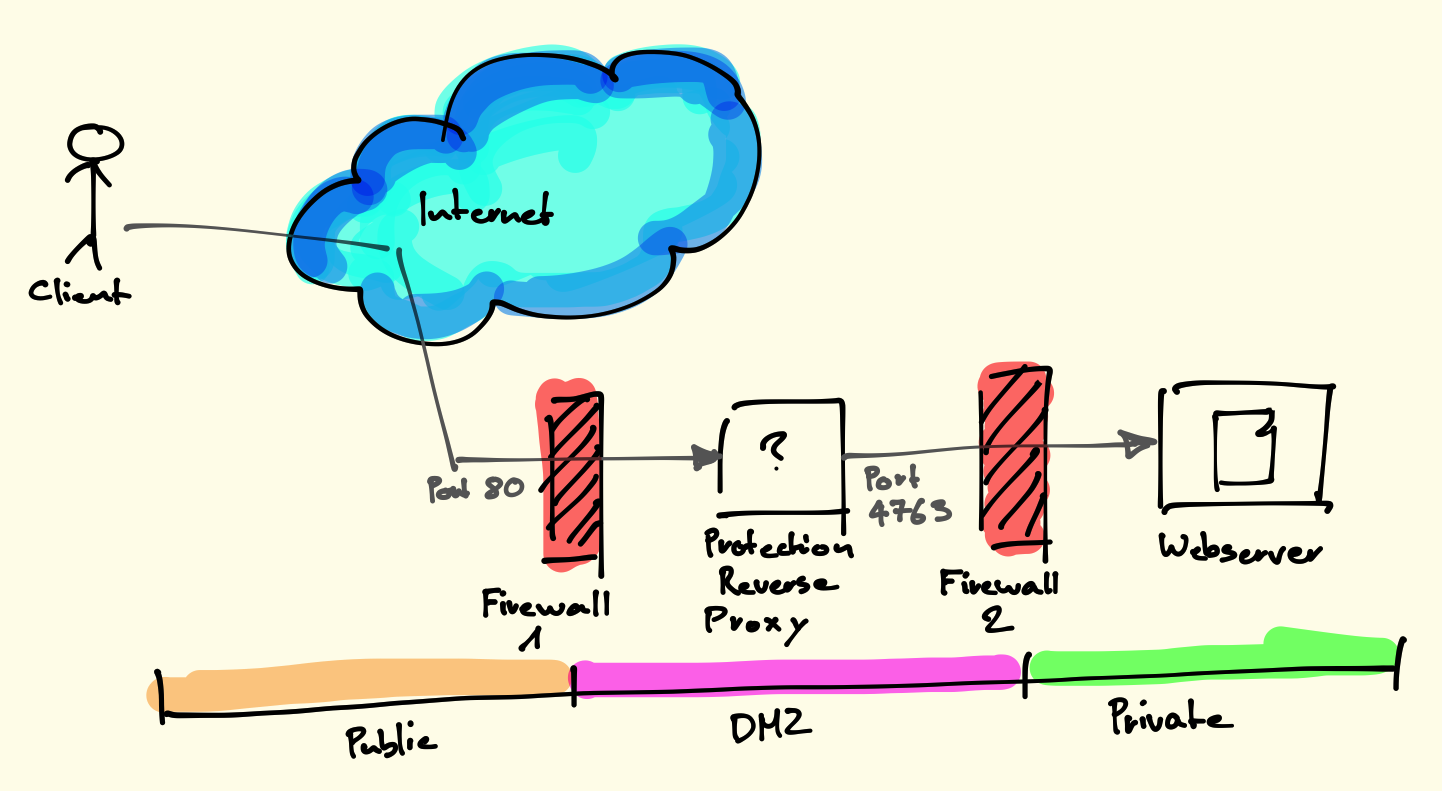
\includegraphics[width=12cm]{content/secure-internet-applications/images/protection-reverse-proxy.png}
	\caption{Strutkureller Aufbau Protection Reverse Proxy}
\end{figure}

\subsubsection*{Ablauf}
Jede eingehende Verbindung wird vom \emph{Protection Reverse Proxy} geprüft und ggf. an den eigentlichen Server weitergeleitet. Sowohl beim Weiterleiten an den eigenen Server als auch beim senden der Antwort an den Client können mit dem \emph{Protection Reverse Proxy} Veränderungen an Header-Fields vorgenommen werden. Das Schreiben von Logs sollte optimalerweise nach dem Versenden der Response geschehen.

Verweigert der Proxy das Weiterleiten eines Requests, ist es von der Sicherheitsrichtlinien abhängig, ob neben dem Senden eines HTTP Statuscodes auch gleich die TCP/IP Verbindung zum Client komplett geschlossen werden soll.

\subsection*{Vorteile}
\begin{itemize}
	\item Web- und Applikationsserver sind für Angreifer nicht mehr direkt erreichbar.
	\item Web- und Applikationsserver können einfacher konfiguriert werden, da diverse Sicherheitsaspekte vernachlässigt werden können. Lediglich der spezialisierte \emph{Protection Reverse Proxy} verfügt über direkte Berührungspunkte mit dem Internet.
\end{itemize}

\subsection*{Nachteile}
\begin{itemize}
	\item Die Verwendung von Blacklist-Filtering suggeriert evtl. eine falsche Sicherheit: Diese Listen verfügen lediglich über bekannte Angriffsmuster.
	\item Verwendet man Whitelist-Filtering, hat man zwar eine grössere Sicherheit, ist aber anfälliger auf infrastrukturelle Veränderungen im eigenen System. Entsprechende Integrationstests sind notwendig und kostenintensiv.
	\item Der \emph{Protection Reverse Proxy} ist eine zusätzliche aktive Komponente im Netzwerk. Dementsprechend leidet die Antwort- und Reaktionszeit.
	\item Clients verfügen über keine End-To-End-Verbindung mit dem eigentlichen Web- oder Applikationsserver mehr. Dies kann als positiv bewertet werden, im Falle von HTTPS oder allgemeinem Session-Handling als zusätzlicher Komplexitätsfaktor angesehen werden.
	\item Fällt der Proxy aus, ist tendenziell das gesamte System nicht mehr erreichbar: Neuer Single Point of Failure.
	\item Hoher Aufwand für Konfiguration und Unterhalt dank erhöhter Komplexität.
\end{itemize}

\subsection*{Mögliche Prüfungsfragen}
\begin{itemize}
	\item \emph{Ist ein Protection Reverse Proxy nur für Webserver, also das HTTP denkbar?}\\
	Nein. Wenn entsprechende Software vorhanden, sind \emph{Protection Reverse Proxies} auch auf anderen Protokollen problemlos machbar. Bspw. könnte ein SMTP \emph{Protection Reverse Proxy} zur Filterung von unerlaubten Befehlen verwendet werden.
\end{itemize}